% Le contexte scientifique prépare la présentation de la mission.

% MIN 2:00 à 3:00. Définir la tâche avant les raisons de la distribuer.
\begin{frame}{Apprentissage supervisé et entraînement distribué}
    En \textbf{apprentissage supervisé}, chaque exemple comprend une entrée
    et la réponse attendue.

    \begin{enumerate}
        \item Le modèle \textbf{prédit une réponse} à partir de l'entrée.
        \item La \textbf{fonction de perte} (\emph{loss}) mesure l'écart
            avec la réponse attendue.
        \item On \textbf{ajuste les paramètres du modèle} pour minimiser
            la perte sur les exemples d'entraînement.
    \end{enumerate}

    \medskip
    \textbf{Pourquoi distribuer l'entraînement ?}\\
    Pour garder les données sur place ou répartir un calcul trop lourd pour
    une seule machine.

    \begin{columns}[T]
        \begin{column}{0.48\textwidth}
            \textit{Claviers de téléphones}\\
            Plusieurs appareils apprennent à prédire le mot suivant sans
            centraliser les textes.
        \end{column}
        \begin{column}{0.48\textwidth}
            \textit{Hôpitaux}\\
            Plusieurs établissements entraînent un modèle de diagnostic en
            gardant les dossiers sur place.
        \end{column}
    \end{columns}
\end{frame}

% MIN 3:00 à 4:15. Lire un tour centralisé, puis définir le décentralisé.
\begin{frame}{Un tour d'apprentissage centralisé}
    Un \emph{worker} est un participant qui effectue un calcul local.

    {\centering
        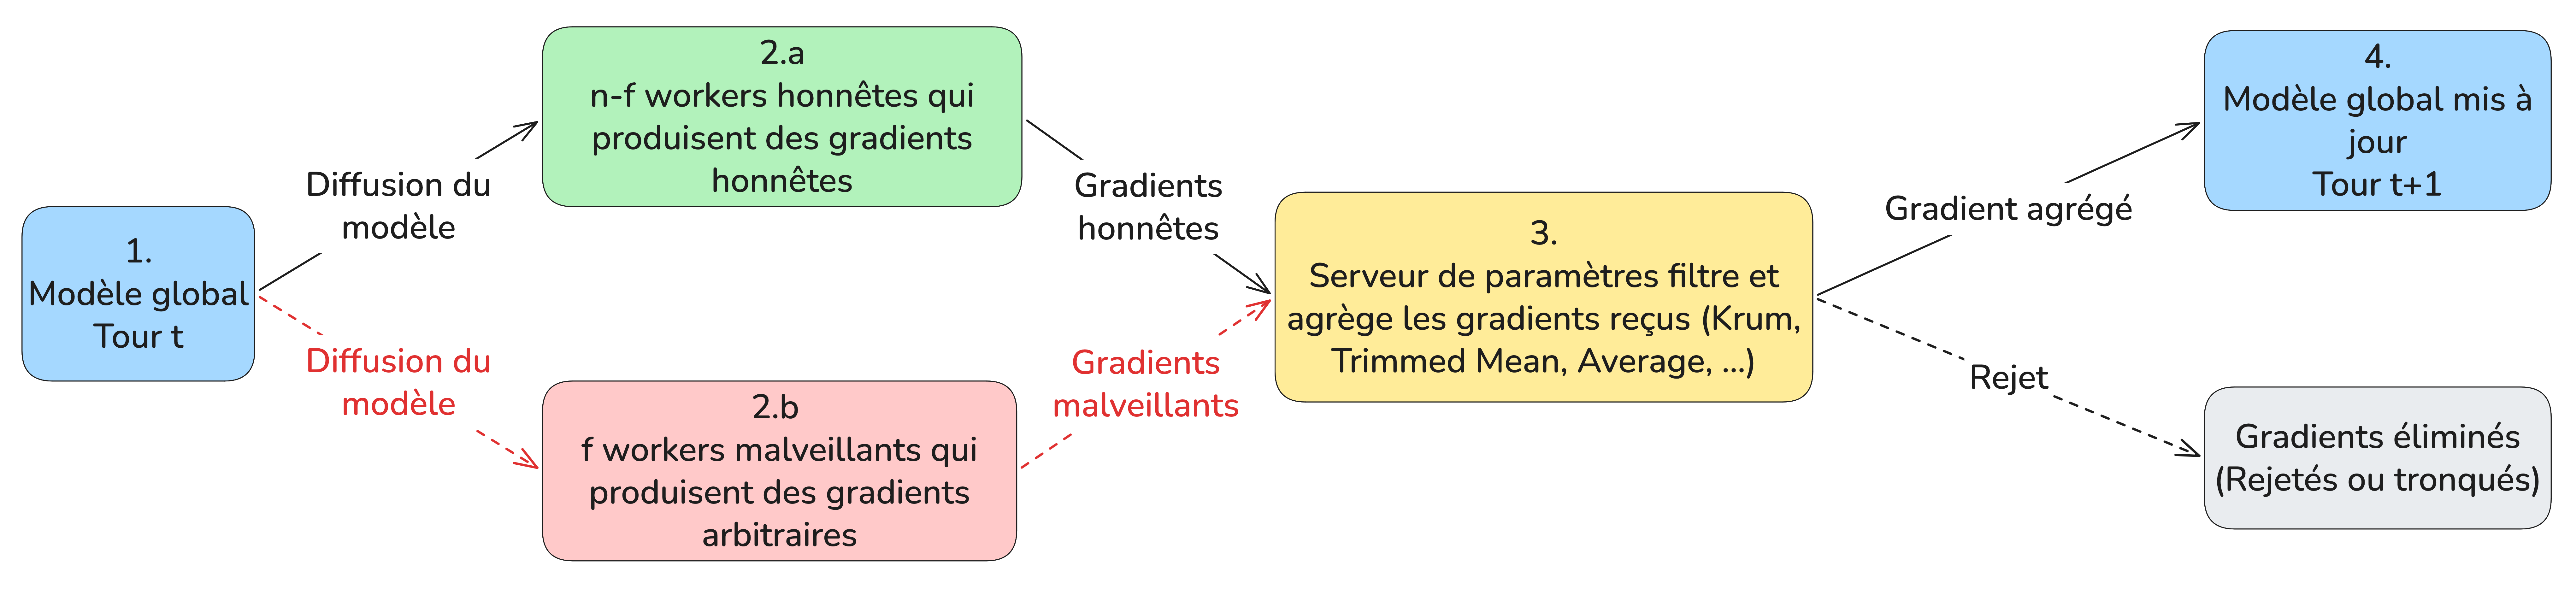
\includegraphics[width=\textwidth]{app-federe-byzantin-centralise.png}
        \par}

    \medskip
    La \textbf{descente de gradient stochastique} (SGD) estime le gradient
    sur un \textbf{mini-lot} d'exemples locaux, puis met à jour le modèle
    dans la direction opposée à ce gradient.

    \medskip
    En \textbf{décentralisé}, les participants mettent à jour leurs modèles
    par des échanges entre voisins, sans serveur central.
\end{frame}

% MIN 4:15 à 5:30. Situer les trois surfaces d'attaque et délimiter le sujet.
\begin{frame}{Des participants malhonnêtes}
    \textbf{Trois surfaces d'attaque}

    \begin{columns}[T]
        \begin{column}{0.30\textwidth}
            \textit{Les données}\\
            L'attaquant altère les exemples.
        \end{column}
        \begin{column}{0.30\textwidth}
            \textit{Le serveur}\\
            L'attaquant compromet le point central.
        \end{column}
        \begin{column}{0.34\textwidth}
            \textbf{Les gradients envoyés}\\
            Des workers malhonnêtes forgent leurs contributions.
        \end{column}
    \end{columns}

    \medskip
    Nous étudions les \textbf{gradients forgés}.
    Dans le \textbf{scénario byzantin}, parmi les $\nworkers$ workers,
    au plus $\nbyz$ sont \textbf{malhonnêtes}.
    Ils peuvent envoyer des vecteurs arbitraires.

    \begin{itemize}
        \item \textbf{Collusion} : les attaquants coordonnent leurs vecteurs.
        \item \textbf{Omniscience} : ils connaissent l'état du système,
            dont les gradients honnêtes.
    \end{itemize}

    Le serveur doit agréger ces vecteurs sans savoir lesquels viennent de
    participants malhonnêtes.
\end{frame}

% MIN 5:30 à 6:30. Montrer l'échec de la moyenne et faire le pont statistique.
\begin{frame}{Pourquoi remplacer la moyenne ?}
    Un attaquant peut déplacer la moyenne aussi loin qu'il le souhaite en
    envoyant un vecteur de grande amplitude dans la direction de son choix.

    Blanchard et al., NeurIPS 2017, lemme 1.

    \begin{block}{Agrégation robuste}
        La règle doit limiter l'influence des attaquants tout en fournissant
        une direction utile à chaque tour d'optimisation.
    \end{block}
\end{frame}
